\documentclass[12pt,spanish]{article}
% aprovechamiento de la p\'agina -- fill an A4 (210mm x 297mm) page
% Note: 1 inch = 25.4 mm = 72.27 pt
% 1 pt = 3.5 mm (approx)

% vertical page layout -- one inch margin top and bottom
\topmargin      -10 mm   % top margin less 1 inch
\headheight       0 mm   % height of box containing the head
\headsep          0 mm   % space between the head and the body of the page
\textheight     255 mm   % the height of text on the page
\footskip         7 mm   % distance from bottom of body to bottom of foot

% horizontal page layout -- one inch margin each side
\oddsidemargin    0 mm     % inner margin less one inch on odd pages
\evensidemargin   0 mm     % inner margin less one inch on even pages
\textwidth      159 mm     % normal width of text on page

\setlength{\parindent}{0pt}

\usepackage{tikz}
\usetikzlibrary{automata,positioning}

\usepackage[doument]{ragged2e}
\usepackage{babel}
\usepackage[utf8]{inputenc}
\usepackage{amsmath,amsthm,mathtools}
\usepackage{amsfonts,amssymb,latexsym}
\usepackage{enumerate}
\usepackage{subfigure, float, graphicx, caption}
\captionsetup[table]{labelformat=empty}
\captionsetup[figure]{labelformat=empty}
\definecolor{RojoAnayelRey}{rgb}{1,.25,.25}
\usepackage[bookmarks=true,
            bookmarksnumbered=false, % true means bookmarks in 
                                     % left window are numbered                         
            bookmarksopen=false,     % true means only level 1
                                     % are displayed.
            colorlinks=true,
            linkcolor=webred]{hyperref}
\definecolor{webgreen}{rgb}{0, 0.5, 0} % less intense green
\definecolor{webblue}{rgb}{0, 0, 0.5}  % less intense blue
\definecolor{webred}{rgb}{0.5, 0, 0}   % less intense red
\definecolor{dkgreen}{rgb}{0,0.6,0}
\definecolor{gray}{rgb}{0.5,0.5,0.5}
\definecolor{mauve}{rgb}{0.58,0,0.82}
\definecolor{MistyRose}{RGB}{255,228,225}
\definecolor{LightCyan}{RGB}{224,255,255}

\begin{document}

\title{Solución al problema 6}
\author{David Cabezas Berrido}
\date{\vspace{-5mm}}
\maketitle

Queremos abrir la cerradura de una caja con las siglas J.N. que hemos
encontrado en las ruinas de Napier. 

\begin{figure}[H]
  \centering
  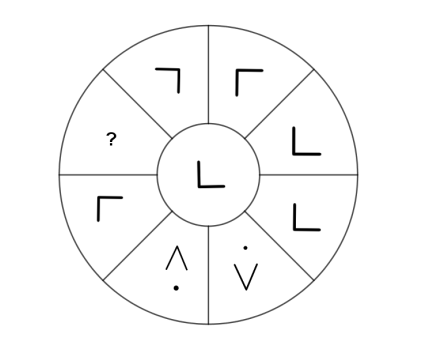
\includegraphics[width=60mm]{6_imagenes/cerradura}
\end{figure}

Para ello debemos dibujar un símbolo en la casilla marcada por ?. La
única pistas que tenemos son estos símbolos grabados en la caja.

\begin{figure}[H]
  \centering
  
\includegraphics[width=120mm]{6_imagenes/simbolos}
\end{figure}

Pues bien, John Napier fue un matemático, físico y astrónomo más
conocido como Ioannes Neper (su nombre latinizado). El logaritmo
neperiano se llama así por el, este es el logaritmo en base $e$. \\

Da la ``casualidad'' de que podemos asignar un dígito a cada símbolo de
tal forma que la secuencia grabada en la caja corresponda a los
primeros decimales del número $e$.

\begin{figure}[H]
  \centering
  \hspace{0.4mm}
  
\includegraphics[width=136mm]{6_imagenes/simbolos}
\end{figure}

\vspace{-10mm}
\[2.\quad 7\quad 1\quad 8\quad 2\quad 8\quad 1\quad 8\quad 2\quad 8\quad 4\quad 5\quad 9\quad 0\quad 4\quad 5\quad 2\quad 3\quad 5\quad 3\quad 6\]

Una vez descifrados los símbolos, la cerradura nos queda del siguiente modo.

\begin{figure}[H]
  \centering
  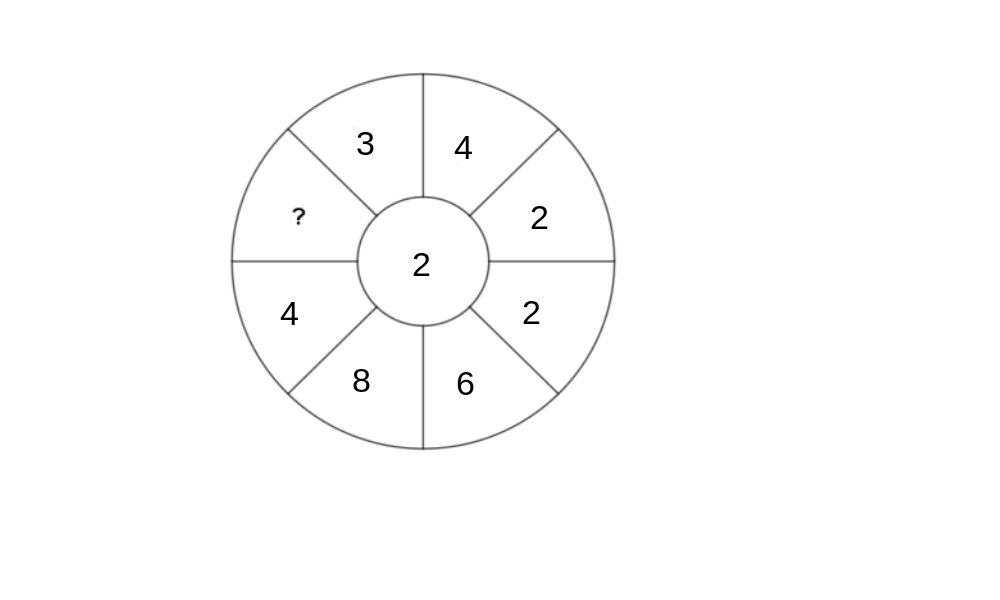
\includegraphics[width=100mm]{6_imagenes/cerradura-resuelta}
\end{figure}

Nos damos cuenta de que cada número de la parte de abajo es el número
de la parte de arriba que hay en frente multiplicado por el del centro
(2), así que hay que dibujar el símbolo correspondiente al 1 en la
casilla desconocida.

\begin{figure}[H]
  \centering
  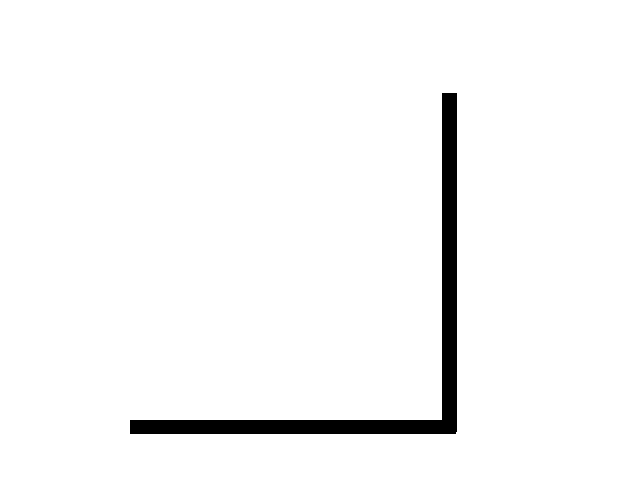
\includegraphics[width=60mm]{6_imagenes/solucion}
\end{figure}

\end{document}